\chapter{Related Work}\label{ch:related}
Simultaneous Localization and Mapping represents a well known complex mathematical problem, based on non-linear optimization. It has been studied by the scientific community since the 80s \cite{durrant2006simultaneous, bailey2006simultaneous}; during this early stage, its statistical formulation has been investigated, proposing interesting results that will constitute, basically, the baseline for all the future SLAM systems.

After some years, in the 90s, the community came-up with early solutions for the SLAM problem. The first systems able to produce appreciable results in terms of speed and accuracy were based on \textit{Extended Kalman Filters} (EKF) \cite{leonard1990dynamic, dissanayake2001solution}. EKFs allow to deal with problem's non-linearity through effective approximations and to represent multivariate distributions with a small number of parameters. This success encouraged the research community to perform deeper investigations in \textit{filtering} approaches \cite{aulinas2008filtering_review}. \textit{Particle filters} started to gain popularity, in particular \textit{Rao-Blackwellized Particle Filters} \cite{grisetti2005improving}: the work of Montemerlo \textit{et al.} \cite{montemerlo2002fastslam} was the first SLAM system able to deal with thousand of landmarks with a good accuracy. 

However, \textit{filtering} approaches revealed not to be the best answer to the SLAM problem due to the computational complexity of the solution, especially when dimensions start to grow. Moreover, system's accuracy is affected by the problem's non-linearities, leading to sub-optimal solutions. For these reasons, \textit{Maximum A Posteriori} (MAP) approaches started to be taken in consideration and the community took a step back to the work of Lu \textit{et al.} \cite{lu1997globally}. Filtering-based approaches align local pose frames incrementally and, thus, different parts of the model are updated independently, generating inconsistencies in the final model. MAP optimization takes into consideration all the local frames and the relations between them at once, leading to a more consistent model and better accuracy. Lu \textit{et al.} embedded all the pose relations into a network with nodes and edges, allowing efficient optimization. However, when they published their work, the computers' computational power was not sufficient to deliver good performance and, thus, this solution was put aside.

Nevertheless, this work represents the precursor to one the most intuitive SLAM formulation, called \textit{graph-based SLAM}, that exploits the computing power of recent robots to deliver impressive performances. In this paradigm, the robot builds an \textit{hyper-graph} whose nodes represent either robot poses or salient points in the world - called \textit{landmarks} - while the hyper-edges encode sensors' measurements between subsets of nodes. 

Graph-based SLAM systems have two main components: \textit{front-end} and \textit{back-end}. The former uses data acquired by robot's sensors to populate the hyper-graph, abstracting raw data into a model that is amenable for optimization. The front-end has to determine the most likely constraint that involves a subset of nodes given an incoming measurement, solving the so-called \textit{data association} problem - \textit{short-term} and \textit{long-term}. Short-term data association has to match corresponding features among consecutive sensor measurements - e.g. stating that visual features detected in multiple consecutive frames represent the same 3D world point. Long-term data association, instead, expresses a more complex problem: it has to associate new measurements to already encountered world points, generating the so-called \textit{loop-closures} - e.g. when a robot passes multiple times across the same place, it has to recognize that it is re-observing the same points in order to generate a map that is consistent with the environment. As for the sensors used, state-of-the-art systems usually acquire data from cameras (RGB or RDB-D) or 3D-LiDARs. The former, in particular, it is gaining much attention from the research community since they are - generally - cheap and can be mounted basically on every electronic device in single or stereo configuration. 

This work, however, focuses on system's back-end, assuming that the given front-end provides consistent estimates. The back-end takes as input the graph and computes the most-likely map given all the constraints. Systems based on this formulation represent the gold standard for map optimization, thus, in the next sections it is proposed a brief overview of the most successful implementations.

\section{Dense Approaches}\label{sec:dense_approaches}
The work of Lu \textit{et al.} \cite{lu1997globally} was the first of its kind: map estimation is obtained through global optimization of the error function deriving from constraints between different poses. They employed a combination of \textit{relation-based} and \textit{location-based} representations, where the former were fixed while the latter were treated as free variables. Those pose-relations were used to construct a network whose nodes were robot poses taken from its trajectory while the constraints between nodes were the pose-relations. Finally, the optimization problem exploits the network to obtain an objective function that will be minimized: the total energy will decrease as the difference between estimated relative pose that involves two nodes and the measured value tends to zero. 

It is good to notice that, in this formulation, the computational power needed for the optimization grows \textit{cubically} with the number of variables involved, thus, it is $O(N^3)$ where $N$ represents the number of poses. Gutmann and Konolige addressed this problem in their work \cite{gutmann1999incremental} proposing a method to incrementally build the network and that determines topologically correct relations between poses.

Those approaches opened the path to a series of study in this direction, that will lead to current state-of-the-art optimizers.

\section{Olson's Gradient Descent}\label{sec:olson}
Evident limitations of the previously seen approaches are that their solution highly depends from the initial estimate of the state. The initial guess is derived from dead-reckoning and, thus, if this is not consistent the system will converge to a local minimum, giving a sub-optimal solution. Olson \textit{et al.} \cite{olson2006fast} addressed this issue, proposing a non-linear optimization algorithm that quickly converges to a good approximation of the global minimum. 

They achieved such results combining two new aspects: the first one is the use of a variant of \textit{Stochastic Gradient Descent} algorithm, which is robust against local minima and has a fast convergence rate; the second one is an \textit{alternative state-space representation} that has good stability and computational properties. This last feature, in particular, allows to update many poses with a relatively small computational cost in a single iteration. Moreover, the memory consumption has been lowered together with the run time - respectively $O(N + M)$ and $O(\log(N))$, where $N$ represents the number of poses and $M$ the number of constraints.

\section{Smoothing and Mapping}\label{sec:sam}
Smoothing and Mapping, shortened as \textit{SAM}, follows the path of global trajectory optimization described in the previous Section. Dellaert \textit{et al.} proposed with \textit{square root SAM} ($\sqrt{SAM}$) \cite{dellaert2006square} a system able to deal with \textit{full SLAM problems}: those require the estimation of the entire set of sensor poses along with the parameters of all the features in the environment. This problem is also known in Photogrammetry as \textit{bundle adjustment} and as \textit{structure from motion} in Computer Vision.

$\sqrt{SAM}$ performs fast optimization exploiting the problem's intrinsic sparsity. Knowing that the measurement Jacobian matrix $A$ is sparse, it is possible to solve the relative linear system in a faster way through a good \textit{variable reordering} together with \textit{QR} or \textit{Cholesky} factorization. For those reasons, $\sqrt{SAM}$ can optimize larger graph without losses in terms of performances or accuracy.

Further improvements were introduced with \textit{iSAM} - \textit{incremental} SAM - developed by Kaess \textit{et al.} \cite{kaess2007isam}. The foundations were the same as $\sqrt{SAM}$, but in this case the system operates incrementally, without the need of fully refactoring the whole QR-decomposition, but updating it every time a new measurement is available. With this solution, it was possible to address real-time problems since the optimization process is faster than before. 

The next iteration of this branch of solutions, is represented by \textit{iSAM2} \cite{kaess2012isam2}. In this case, a new data-structure is proposed, the \textit{Bayes tree}, to map better the square root information matrix of the problem. Employing Bayes trees, the algorithm is able to further improve the performances, exploiting incremental variable re-ordering and fluid relinearization, eliminating the need for periodic batch steps. 

\section{TORO}\label{sec:toro}
Grisetti \textit{et al.} proposed in their work TORO \cite{toro} - Tree-based netwORk Optimizer - an extension of Olson's algorithm to efficiently manage 2D and 3D graph-based optimization problems. 

This frameworks has several features that allow it to achieve good performances in terms of speed and accuracy. The first one is a revisited version of the standard \textit{Stochastic Gradient Descent} used to perform the optimization process, together with a technique to efficiently distribute the \textit{rotational error} over a sequence of 3D poses \cite{grisetti2007efficient}. In fact, due to the non-commutativity of rotational angles in 3D, major problems may arise when applying approaches that are designed for a 2D world. As a result, TORO converges by orders of magnitude faster with respect to previous approaches.

Moreover, it employs a \textit{tree parametrization of the nodes} \cite{grisetti2007tree} that significantly improves the performances and allows to deal with arbitrary network topologies. This consented the authors to bound algorithm complexity to the size of the mapped area and not to the trajectory's length, yielding accurate maps of the environment in a small amount of time.

\section{G2O}\label{sec:g2o}
The work of K\"ummerle \textit{et al.} \cite{kummerle2011g} is an open-source C++ frameworks for optimizing \textit{non-linear least squares problems} that can be represented as a graph. Its generality together with a cross-platform implementation made \texttt{g2o} one of the most successful graph optimization tool, which is employed in many state-of-the-art full SLAM systems. 

This work focuses on efficiency, which is achieved at various levels: it exploits graph sparsity and takes advantage of the graph's special structure to perform fast optimization; it uses advanced methods - Cholesky decomposition through CHOLMOD library - to solve sparse linear system; finally, it utilizes modern processor's features to perform fast math operation optimizing cache usage - e.g. SIMD instructions. Moreover, this frameworks offers the possibility to choose between different algorithms - i.e. Gauss-Newton, Levenberg-Marquardt - and linear solvers - direct and iterative.

Our approach still delivers comparable performances with respect to \texttt{g2o} while being lightweight and more simple to include in a full SLAM pipeline. In fact, \texttt{g2o} is a big framework, with over 40 thousands lines of code and, thus, its inclusion may add weight to the system.

\section{GT-SAM}\label{sec:gtsam}
GT-SAM is a C++ library developed by Dellaert \textit{et al.} \cite{dellaert2012gtsam} at the Georgia Institute of Technology, which provides solution to a wide range of SLAM and Structure From Motion (SfM) problems, based on factor-graph optimization. It provides both C++ and MATLAB implementations that allow to easily develop and visualize problem solutions. 

This work - like it has been previously seen in \g2o - also focuses on efficient optimization and takes advantage of the graph sparsity to deliver fast and accurate performances. However, this framework is even more big and complex - over 300 thousands lines of code - making it very difficult to unravel and understand what is under the hood.

\section{HOG-Man}\label{sec:hogman}
Grisetti \textit{et al.} in their work \cite{grisetti2010hogman} proposed an optimization system designed for accurate, fast and memory efficient on-line operations: \textit{HOG-Man} - which stands for Hierarchical Optimization on Manifolds.

\begin{figure}[!hbt]
    \centering
    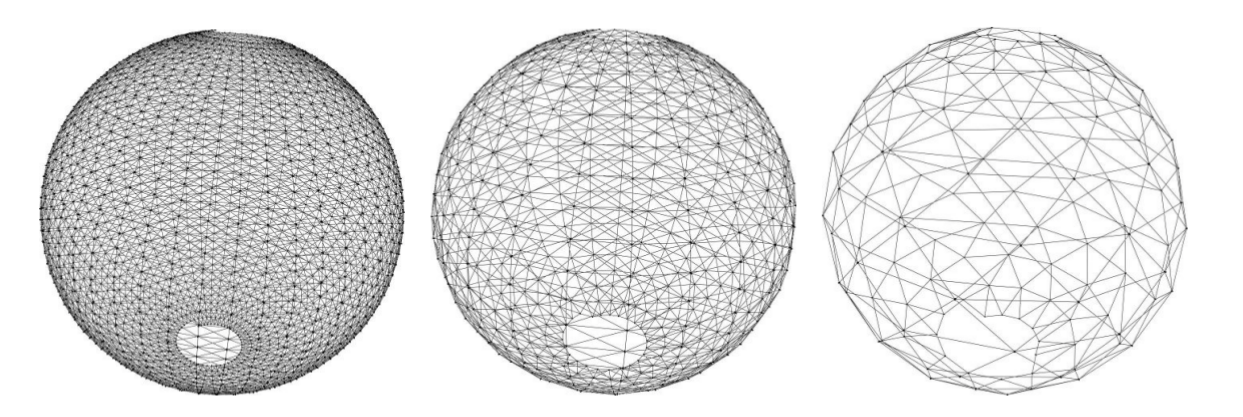
\includegraphics[width=\textwidth]{figures/01_related/hogman.png}
    \caption{\textbf{HOG-Man.} The image - courtesy of \cite{grisetti2010hogman} - sketches the idea behind this approach: the systems creates multiple "views" of the graph's structure, each with a different level of abstraction. Proceeding from left to right it is shown the original structure - i.e. the bottom of the hierarchy - a mid level representation and the final structure - i.e. the top of the hierarchy.} 
    \label{fig:hogman}
\end{figure}

At its core there is a \textit{hierarchical} approach to graph optimization: during on-line mapping, it optimizes only the coarse structure of the environment and not the whole map. The simplified problem that is solved, however, contains all the relevant information to let the front-end solve properly the data association problem. 

It is good to notice, that there are \textit{different level of abstractions}: the bottom is the original input, while higher levels are always more compact. When the top levels are modified, only portions of the underlying ones are updated, namely the ones subject to consistent modifications. This method limits the computational power needed for on-line operations while preserving global consistency, outperforming several previous approaches.

\section{Tectonic-SAM}\label{sec:tsam}
Ni \textit{et al.} propose a way to reduce the computational effort due to the linearization update, based on sub-map partitioning: \textit{Tectonic SAM} \cite{ni2007tectonic} - shortened as \textit{T-SAM}.

The original problem is addressed through a \textit{divide and conquer} approach which produces local sub-maps. Those smaller maps are individually optimized and then the local linearization can be cached and reused when sub-maps are combined into a global map, speeding up the linearization process. Sub-maps have a base node that capture their global position and the authors showed that, under \textit{mild assumptions}, this approach leads to the exact solution. 

The next iteration - called T-SAM2 \cite{ni2010nestedDiss} - proposes an algorithm that partitions the SLAM factor-graph into a sub-map tree, performing the optimization from leaves to root. In T-SAM, partitioning was done using edge separators; moreover, T-SAM was not able to maintain hierarchical maps, leading to poor scalability with respect to larger datasets. All those problems were addressed in T-SAM2, where partitioning is done employing the \textit{nested dissection algorithm} that, together with a novel \textit{multi-level} approach, provides a more efficient and robust exact solution.

\section{Condensed Measurements}\label{sec:cmeas}
The solution of least-squares problems that can be represented as factor-graph - like in SLAM and SfM - is contingent to both \textit{initial estimate} and \textit{sensor models' non-linearities}. Grisetti \textit{et al.} proposed a way to enlarge the convergence basin based on the \textit{divide and conquer} approach that exploits the factor-graph's structure \cite{grisetti2012condensed}. 

The core of this formulation is to divide the graph into \textit{small locally connected sub-graph}, each of which represents a sub-problem that can be robustly solved - like it has been suggested in previous systems like HOG-Man \cite{grisetti2010hogman} and T-SAM \cite{ni2010nestedDiss}. In order to consistently combine the local sub-graphs, the authors build a simple factor-graph from the sub-graphs, constraining the relative positions of the variables in the solution. For this reason, the sub-graphs are called \textit{condensed measurements}. The resulting problem is more convex with respect to the original one and, thus, there are more chances of finding the correct minimum that can be used as initial guess for standard minimization algorithms - e.g. Levenberg-Marquardt.

This formulation allows to recover from bad initial estimations, where most of the other approaches fail - both batch and direct ones - but, unfortunately, it does not deliver real-time performances.

